\documentclass[12pt]{article}
\usepackage{graphicx}
\pagestyle{plain}

\oddsidemargin  -0.5 cm
\evensidemargin 0.0 cm
\textwidth      6.5in
\headheight     0.0in
\topmargin      -1 cm
\textheight=9.0in

\title{Tools for ZD/DR Alignment}
\author{Jim Pivarski}
\date{\today}

\begin{document}
\begin{figure} \flushright CBX 04-4 \end{figure}

\maketitle

\abstract{Two suez modules to facilitate alignment, ZDAlignmentMod and
  DRAlignmentMod, are presented in three levels of detail: strategy,
  use, and implementation.  DualTrackProd, a suez producer which
  implements a two-track (bhabha, $\mu$-pair) constraint is also
  described, on the level of use.  Three related processors/producer
  are also explained: ZDAlignmentBhabhaFilterProc,
  DRAlignmentBhabhaFilterProc, and DualTrackToUsageTagProd.  This
  document is intended for anyone who will be globally aligning the ZD
  or aligning DR wedding cake rings, and will assume familiarity with
  suez.  An alignment strategy will be described in detail, but
  current issues in and obstacles to alignment are not presented in
  this note.}

\pagebreak
\tableofcontents

\section{Quick Introduction}

For centuries, mankind has gazed into the stars and pondered how to
align the ZD.  ZDAlignmentMod is a code package that I developed to
encapsulate the latest ideas on how to do this, and to automate the
process once it's fully understood.  DRAlignmentMod and DualTrackProd
are offshoots which will probably be useful as well, for aligning the
DR wedding cake (DRAlignmentMod) and for getting pairs of tracks which
are constrained to be back-to-back (DualTrackProd), {\it with
residuals.}  Each will be described in a major section of this note.

ZDAlignmentMod and DRAlignmentMod are intended as works in progress:
as tracking problems become understood, it will probably be necessary
to change (or re-write) the code.  On the other hand, DualTrackProd
does a simple thing, and I think it does it correctly.  Therefore,
while the implemenation of the two alignment modules will be fully
exposed in this document, the dual-track producer will only be
explained from a user's perspective.

\section{ZDAlignmentMod {\normalsize (and ZDAlignmentBhabhaFilterProc)}}

\subsection{ZDAlignmentMod Strategy}
\label{ZDAlignmentMod_Strategy}

``ZD or DR Alignment'' here means to find the real orientation of the
ZD, or of subcomponents of the DR, relative to the DR stereo section
which defines the CLEO coordinate system.  The true orientation may be
different from the orientation assumed in track reconstruction, which
may lead to tracking biases.  These kinds of biases are easiest to see
in bhabha or $\mu$-pair events, where the final state is easy to
anticipate: two nearly straight tracks originating from a common
point, recoiling at beam energy in opposite directions.

For ZD alignment, we are interested in determining the orientation of
a small detector (the ZD) with respect to a large, existing one (the
CLEO-III central drift chamber).  We can do this most cleanly by
telling the track fitter to not use ZD hits in the track fit.  We
still want to know which hits are associated with a given track (which
is a part of track finding), and we will want to calculate how close
the fitted track comes to the those ZD hits.  These differences are
known as ``residuals'' and are defined as the distance of closest
approach of the electron's or muon's track to the wire, measured by
drift time (here usually called ``drift''), {\it minus} the
reconstructed helix's prediction of that distance (distance of closest
approach, or ``dca'').  The distribution of these residuals, plotted
with respect to $\theta$ or $\phi$, can usually be interpreted as a
geometric misalignment.

This is what ZDAlignmentMod does: it loads into memory a large sample
of bhabha tracks, fit only to DR hits, along with their associated ZD
hits.  For a given trial ZD alignment, it will plot distributions of
residuals as functions of $\theta$, $\phi$, drift, and ZD layer.  If
the user sees an obvious misalignment in these plots, e can adjust the
alignment parameters until the deviations are minimized.
ZDAlignmentMod also calculates the total root mean square residual and
passes that value to MINUIT, so that MINUIT can automatically adjust
alignment parameters to find the precise minimum.  If the ZD
calibration (drift functions and T0s) is also correct, this procedure
will find the correct ZD alignment, and the RMS residual will be the
intrinsic resolution of the ZD.

\subsubsection{Dual-Track Constraint}
\label{dualconstraint}

The tracks used are ``dual-constrained,'' that is, we take advantage
of the back-to-backness and common origin of bhabha electrons as an
additional constraint in their fit.  After the two tracks have been
fitted to the DR and assigned error matrices, we find the optimal
track-pair which satisfies these relations:
\begin{itemize}

  \item the impact parameters $d_0$ (X-Y plane) and $z_0$ are the same
  for each track (with opposite signs for $d_0$),

  \item the total transverse momentum is consistent with crossing
  angle (incident beams are crossed a few milliradians in the XZ
  plane), and

  \item the total longitudinal momentum is zero, because CESR collides
  beams of equal energy.

\end{itemize}
This dual-track is obtained from the two fitted tracks by shifting
their least well determined parameters most, and a $\chi^2$ for the
dual fit represents the consistency of the two original tracks with
the result.  Most often when the two tracks are inconsistent with the
resulting dual-track (the dual-$\chi^2 \gg 1$), it is because they had
to be tilted too much in $\theta$ to satisfy the longitudinal momentum
constraint.  This is not surprising, as bhabhas can radiate a photon
in the initial state, and this momentum loss is usually along the beam
axis.  The $\chi^2$ from the dual-constraint is used to select bhabhas
with little radiation.

Dual-tracks are preferred for ZD alignment because track projections
to the ZD are an interpolation in the middle of a dual-track, but
extrapolations on the end of an ordinary singly-fitted track.  Since
the dual-track is constrained by DR hits on both sides of the ZD, the
dual-track has a smaller error on an event-by-event basis and an
additional symmetry which might cancel unknown biases in DR track
fitting.  To get dual-tracks for other applications, the algorithm has
been packaged into DualTrackProd (see Section \ref{dualtrackprod} on
page \pageref{dualtrackprod}).

\subsubsection{Use ChisqFitProd for tracks}
Another strategy to reduce DR track fitting biases is to use
ChisqFitProd, rather than the usual Kalman fitter.  ChisqFitProd fits
tracks to simple helices by minimizing their $\chi^2$, and doesn't
have a hit-order dependence like the Kalman fitter does.  (One bias
was observed in ZD residuals relative to Kalman fits: tracks that
passed through a different number of DR superlayers had systematically
different ZD residuals.  This bias was not present in
ChisqFitProd-fitted tracks.)

\subsubsection{Bhabha Event Selection Criteria}
An auxiliary processor, ZDAlignmentBhabhaFilterProc, was built to
define bhabha events.  The cuts are typical, but chosen to be tight.
We require:
\begin{itemize}
  \item exactly two ``good tracks,'' with oppositely-signed charge,
  \item $|(d_0)_1 + (d_0)_2| <$ 0.5 mm,
  \item $|(z_0)_1 - (z_0)_2| <$ 1.5 cm,
  \item $(\vec{p}_1 + \vec{p}_2)_\perp <$ 2\% of beam energy, and
  \item $(\vec{p}_1 + \vec{p}_2)_\parallel <$ 2\% of beam energy.
\end{itemize}
A ``good track'' is defined as one which:
\begin{itemize}
  \item successfully fit,
  \item with $\chi^2/\mbox{\sc Dof} <$ 10,
  \item number of layers hit / expected between 0.5 and 1.2,
  \item $|d_0| <$ 5 mm,
  \item $|z_0| <$ 5 cm,
  \item $|\vec{p}|$ between 90\% and 110\% of beam energy,
  \item $|\cot \theta| <$ 2.4,
  \item ${\sigma_{\cot \theta}}^2 <$ 0.5 $m^2$ and
        ${\sigma_{z_0}}^2 <$ 0.25 m$^2$,
  \item with at least one ZD hit.
\end{itemize}
ZDAlignmentMod additionally requires $|\cot \theta| <$ 2 and a
dual-$\chi^2$ $<$ 20.  This last cut removes many bhabhas with initial
state radiation.  (This doesn't introduce a bias because CLEO-III sees
the same distribution of +Z ISR bhabhas as -Z ISR bhabhas.)

All of these selections are made to tracks which {\it did not} include
ZD hits in the fit.

\subsubsection{ZD Hit Corrections}

After ZD hits have been associated with a track, they are additionally
corrected for the bhabha electron's flight time from the origin to the
hit location and the time for the signal to propogate along the ZD
wire.  These are nanosecond-scale corrections on 0.1 microsecond drift
times, and involve no tunable constants.  They are applied in
ZDAlignmentMod, just before calculation of the residual.

\subsubsection{ZD Hit Selection Criteria}

Right now, ZDAlignmentMod also removes some ZD hits before plotting
them or using them for alignment optimizations.  Hits are dropped if
they are labled by the track finder as {\tt kDO\_NOT\_FIT}, all hits
on layers 1 and 6 are dropped (edit ZDAlignmentMod.cc:609 to change
this), hits closer than 1.5 mm or further than 3.8 mm to the wire are
dropped (set the parameters minDrift and maxDrift to change this), and
a few wires are singled out as bad and therefore dropped (edit
ZDAlignmentFcn.cc:357 to change this).
\begin{center}
  \begin{tabular}{c | c}
    Layer & \hspace{0.5 cm} Bad wire (as numbered by {\tt wireInLyr()}) \hspace{0.5 cm} \\\hline
    4 & 1, 5, 6, 8, 27, 31, and 43 \\
    5 & 19 and 54; \\
    6 & 11 \\
  \end{tabular}
\end{center}

\subsection{ZDAlignmentMod Use}

Even though these modules might someday find their way into a fixed
release, it is a good idea to check them out of the repository so that
you can make changes to the code.  For ZD alignment, check out
ZDAlignmentMod and ZDAlignmentBhabhaFilterProc.  If you are using the
Oct15\_03\_MC release or earlier, you will also need to check out
HbookHistogram and HbookHistogramModule to get a necessary bug fix to
histogram resetting.  (Compile HbookHistogram first.)  The Qt version
(how the interactive histograms look) also changed after Oct15\_03\_MC,
so you can pick your favorite.

\subsubsection{Running ZDAlignmentBhabhaFilterProc}

The alignment process has been split into two stages for efficiency:
DR track finding/fitting, and ZD hit residual calculation.  The first
stage is run once: fill PDS files with ZD hits and DR tracks in batch
jobs using ZDAlignmentBhabhaFilterProc, massively in parallel.  The
second stage is done inside ZDAlignmentMod iteratively, using
different trial alignments.  So before you can do an alignment, you
need to set up many jobs to collect tracks and hits, and possibly run
them overnight.  Look in ZDAlignmentBhabhaFilterProc/Test/sample.tcl
for hints in setting up your tcl files.  The key issues you will need
to keep in mind are:
\begin{itemize}
  \item Use the DR/ZD calibration of your choice, including the latest
  fittingweights, when they become available.

  \item Select ChisqFitProd, rather than KalmanProd.  This is tricky
  if you are using \$C3\_SCRIPTS/trackingDataFull.tcl, since it
  automatically loads KalmanProd.  Do this for safety:
  \begin{verbatim}
prod sel ChisqFitProd
run_file $env(C3_SCRIPTS)/trackingDataFull.tcl                                         $
prod desel KalmanProd \end{verbatim}
  It is important to load ChisqFitProd's symbols before KalmanProd
  gets a chance to load its own, so that you can be sure it really is
  ChisqFitProd that is running.

  \item To remove ZD hits from track fitting, use this trick:
  \begin{verbatim}
param ChisqFitProd ForceZDFittingWeight true
param ChisqFitProd ZDFittingWeight 1e-10 \end{verbatim} \label{fittingweights}
  Technically, the ZD hits are still used in the track fit, but their
  weight is so small that it doesn't matter.  One could also inflate
  the values in the constant ZDWeight2LayerDriftEntAng: this would
  have the same effect.  (The ``fittingweight'' given as a parameter
  is loose when small, while the ``fittingweight'' given in
  ZDWeight2LayerDriftEntAng is loose when large.  This is a failure of
  our terminology: the values in ZDWeight2LayerDriftEntAng are
  actually resolutions, in units of length, while the ChisqFitProd
  parameter takes a weight, in units of 1/length$^2$.)

  There are another two parameters, UseZDStereoU and UseZDStereoV, but
  these will actually remove the hits from the track lattices so they
  can't be found by ZDAlignmentMod for residual calculations.  Don't
  use them.

  \item These additional producers will be necessary to do tracking on
  ZD data:
\begin{verbatim}
prod sel AZDGeomProd
prod sel ZDGeomProd
prod sel CalibratedZDHitProd
prod sel ZDDriftFunctionProd
prod sel ZDHitCorrectorProd
prod sel CesrBeamEnergyProd
prod sel DBEventHeaderProd

param DetectorConfigurationProd Override true
param DetectorConfigurationProd UseZDnotSI true
param DRHitCorrectorProd ApplyEntranceAngleCorr true
param DRHitCorrectorProd ApplyStandardCorrections true \end{verbatim}
  I expect trackingDataFull.tcl will soon include these, with the
  possible execption of the DR hit corrections.  (In the CLEO-III
  trackingDataFull.tcl, DR hit corrections were turned off by
  default.)

  \item Include enough data for ZDAlignmentMod to be able to run.  The
  minimum set of objects is
  \begin{itemize}
    \item FAItem$<$DBEventHeader$>$
    \item FAItem$<$DBTrackerValues$>$
    \item FATable$<$TRTrack$>$
    \item FATable$<$TRHelixPionFit$>$
    \item FAItem$<$SeedTrackZDHitLattice$>$
    \item FATable$<$CalibratedZDHit$>$
  \end{itemize}
  Tcl code to do this is provided in
  ZDAlignmentBhabhaFilterProc/Test/sample.tcl, though this includes
  more data in the PDS file than the minimal set above.

  (This was part of an attempt to include enough data in the PDS files
  to reconstruct ZD hits at the ZDAlignmentMod level (so that the user
  doesn't need to re-run tracking to include new ZD calibrations).  I
  haven't found a way to get it to work, but it is a worthwhile goal.)

\end{itemize}

\subsubsection{Running ZDAligmentMod}

Once you have a repository of fitted tracks on a large disk somewhere,
alter ZDAlignmentMod/Test/align.tcl such that it points to your PDS
files.  With early CLEO-c run lengths and cosmic ray backgrounds, four
runs will give you enough data for an exploratory alignment (meaning:
you have to wait ten seconds between iterations--- the limit of my
interactive patience).

You will need to set an initial ZDGeomAlignment file, e.g.\ from the
database: \label{constantsweb}
\begin{center}
{\tt http://www.lns.cornell.edu/restricted/CLEO/CLEO3/soft/Constants/},
\end{center}
and point ZDAlignmentMod at it using the ``geom'' parameter.  Because
I didn't remove all of my experiments, you will also need to fill a
file named {\tt normal.azdgeomlayer} with the default values of
AZDGeomLayer.  ZDGeomAlignment is the one that contains ZD alignment
information; AZDGeomLayer defines things like wire layer radii and
should not be changed.  (If you don't want to call it
{\tt normal.azdgeomlayer}, you will need to set ZDAlignmentMod's
``geomLayer'' parameter.)  If you use the above website to get a
constants file, it probably set the validity range (first two numbers)
to ``0 0'' (valid for no runs).  Set it to ``1 0'' (valid for all
runs).

Now run {\tt suez -f align.tcl}.

Once suez has loaded everything, type {\tt iterator go}.  This opens a
HistogramViewer window with seven plots to help you with alignment.
Close the ``instructions'' subwindow (those instructions don't apply
to ZDAlignmentMod, anyway) and open histogram subwindows with the
heirarchy on the left by double-clicking.  Arrange the subwindows now,
becuase unlike HistogramViewerProc, you won't get a chance to move
them again later.  The ``Update Frequency'' field is meaningless for
ZDAlignmentMod, as is the ``Interact'' button.  The ``Continue''
button is used once: after you are happy with the arrangement of
histograms and would like to start aligning.

Once you press ``Continue,'' the module will load the tracks and hits
from the PDS files and store them in memory.  This is the last massive
memory allocation: if you don't have enough memory, the module will
crash here, not later.  Once everything is loaded, MINUIT will go into
interactive mode.  From here, any MINUIT command may be executed.

MINUIT's function FCN is set to do the following:
\begin{itemize}

  \item For each (dual-constrained) track, project the track into the
  ZD and calculate the residual difference between measured and
  predicted drift distance, using the current trial ZD geometry.

  \item Fill profile histograms that plot this residual as a function
  of $\theta$, $\phi$, drift, and ZD layer.

  \item Calculate the root-mean-square residual in millimeters and
  serve this as FCN's return value.

  \item Draw all of the plots in the HistogramViewer window.

\end{itemize}
Unfortunately, it is not easy to add commands to MINUIT to break up
these functions into separate commands, so if a window (or a
screensaver) covers the HistogramViewer window, you will need to
recalculate all residuals to redraw the plots.  Also, MINUIT doesn't
call FCN unless it expects FCN's return value to change, so sometimes
you may need to set a parameter value without changing it to force a
redraw.

Interactive MINUIT commands are documented on this webpage:
\begin{center}
\tt http://wwwasdoc.web.cern.ch/wwwasdoc/WWW/minuit/minmain/chapter2\_8.html
\end{center}
but the most useful ones are these:
\begin{itemize}

  \item {\tt show par} --- Print current parameter values and call FCN

  \item {\tt set par $N$ $x$} --- Manually set parameter number $N$ to
  value $x$.

  \item {\tt fix $N$} --- Freeze a parameter so that it won't be
  varied in automatic optimization.

  \item {\tt rel $N$} --- Release a parameter for automatic
  optimization.

  \item {\tt mini} --- Let MINUIT vary all free parameters to minimize
  FCN, the root-mean-square residual.  This does a little more than
  you want: it calculates ``errors'' for each parameter as though the
  RMS residual were a $\chi^2$.

  (This is why residuals are reported in millimeters: the residual RMS
  should be $\mathcal{O}(1)$ like a $\chi^2$.  If residuals were
  reported in meters, MINUIT would take longer to calculate the
  meaningless ``errors.'')

\end{itemize}

\subsubsection{How to interpret the MINUIT parameters}

There are thirteen parameters, but normally you should only use the
first six.  These six describe the orientation of the ZD detector, in
this order:
\begin{enumerate}

  \item {\bf x} is the offset of the ZD with respect to the center of
  the DR stereo section, in the direction parallel with the ground and
  perpendicular to the beamline.  MINUIT is given this parameter in
  millimeters, so if you {\tt set par 1 0.1}, you will set {\bf x} to
  100 microns, not 10 centimeters.  (Positive offsets are away from
  the CESR ring, negative ones are toward the ring's center.  Not that
  it matters.)

  \item {\bf y} is the vertical ZD offset, also in millimeters, with
  up being positive.

  \item {\bf z} is the offset along the beamline (in the direction
  that the CESR positrons travel).  It will be the most poorly
  determined of the translations, since it is measured only through
  the ZD stereo angle.

  \item {\bf phix} is the angle that the ZD makes with respect to the
  X axis.  If the ZD were an airplane, {\bf phix} would be the pitch.
  The angles are presented in milliradians.  Another way to think of
  this parameter is that a nonzero {\bf phix} is a +{\bf y} offset on
  one ZD endcap, and a --{\bf y} offset on the other.

  \item {\bf phiy} is the angle that the ZD makes with respect to the
  Y axis, also in milliradians.  It can also be called the yaw, or an
  antisymmetric offset in {\bf x} on the ZD endcaps.

  \item {\bf phiz} is the angle that the ZD makes with respect to the
  Z axis, or the roll.  Unlike the other two angles, this one is in
  the X-Y plane and is therefore most easily measured.

  In principle, one would need to worry about which order these
  rotations are applied in the code, since they don't commute.  In
  practice, though, these corrections are small (less than 0.01
  radians), so any alignment on a fine enough scale for this to matter
  would be done with a MINUIT minimization, anyway.

\end{enumerate}

Because suez expresses all lengths and angles in meters and radians
while ZDAlignmentMod expresses them in millimeters and milliradians,
ZDAlignmentMod always multiplies by a thousand when reading them in
from constants and divides by a thousand when writing out to constants
or when telling suez what to do with them.  This is handled correctly.

The remaining parameters were implemented as experiments, and then
never removed.  Most of these will not be useful, and you may remove
them if you are desperate for screen space.
\begin{enumerate}\setcounter{enumi}{6}

  \item {\bf t0}

  \item {\bf drift} If the parameter ``fakeDriftFunction'' is set to
  true, ZD drift measurements won't be taken from {\tt distance()},
  which includes all calibrations and corrections, but from {\tt
  time()}, the raw drift time.  {\bf t0} and {\bf drift} are the
  offset and slope of a linear drift function.  This may be used as a
  cross-check if you are afraid that the drift functions are hiding
  alignment issues.

  \item {\bf radius}
  \item {\bf del\_rad\_45} One can artificially change the slope of a
  residual versus $\cot(\theta)$ plot by adjusting the assumed radius
  of all wires in the chamber.  Don't do this.

  The second parameter, {\bf del\_rad\_45}, allows you shift the radii
  of wires in U layers differently from those in V layers.  Don't do
  this either.

  \item {\bf sagx}
  \item {\bf sagy} These adjust the gravitational sag of wires in the
  X and Y directions.  (It takes some imagination to explain a sag in
  the X direction, but CESR is built into a hill\ldots)  The default
  sag is zero, as it should be too small to measure in either
  direction.

  \item {\bf twistWest} allows the user to apply a different {\bf
  phiz} on the west endplate than the east--- an {\it internal}
  alignment of the ZD.  The default value of this parameter is nonzero
  because the internal alignment has already been fixed.

\end{enumerate}

\subsubsection{How to interpret the plots}

Only one of the seven plots is a one-dimensional histogram: {\bf
resid} plots the number of hits per ZD residual bin.  It should be
narrow and roughly Gaussian, with an RMS of about 0.1--0.2 mm.  For
internal consistency, all residuals are reported in millimeters, even
in the plots, so the numbers on the horizontal axis are also in
millimeters.  (This also saves screen space, since 1, 2, 3 takes less
room than 0.001, 0.002, 0.003.)  In pathological cases, this plot
might have a wide, flat-topped peak if the ZD is not properly aligned,
two or more peaks if it is way out of alignment, or a long tail if a
necessary correction is being ignored, for example.

All of the other plots are profile histograms, and all vertical axes
are ZD residuals in millimeters.
\begin{itemize}

  \item ``V ndrift'' plots residuals versus normalized drift distance.
  (``V'' always means ``ZD residual versus.'')  The normalized drift
  distance is the measured drift in units of the cell width.  (Bins
  $\pm$1 are filled with hits at the edge of the drift cell, 0 with
  hits very close to the wire, etc.)  A {\bf phiz} rotation can
  vertically raise and lower the entries in this plot, but it is
  mostly intended to diagnose the problems with T0s (a calibration
  issue).  A gap between positive and negative drift distances
  indicates a global T0 problem.

  \item ``V layer'' plots residuals versus layer number.  A gap
  between layers 2, 3 and layers 4, 5 indicates a {\bf Z} offset,
  since the first three layers have a different stereo angle from the
  last three layers.

  \item ``V cotTheta'' plots residual versus track $\cot(\theta)$,
  or, for a given layer, residual along the length of the wire.  A
  track with $\cot(\theta) = 0$ points directly into the barrel,
  $\cot(\theta) = \pm 1.49$ points into the corner of the barrel
  region, and $\cot(\theta) = \pm 2$ is the furthest into the endcap
  that DR Z measurement can be trusted.

  Solving outstanding problems in ZD alignment will probably involve
  doing something with this plot.  There is a slight (100 micron)
  bowing in {\it timelike} residuals versus $\cot(\theta)$--- this
  indicates that some ZD hit corrections are not being applied
  correctly.  I don't know why there's a slope in spacelike residuals
  versus $\cot(\theta)$.

  \item ``V phi (--theta)'' plots residual versus $\phi$ for $-2.0 <
  \cot(\theta) < -1.4$.
  \item ``V phi (0theta)'' plots residual versus $\phi$ for $-1.4 <
  \cot(\theta) < +1.4$.
  \item ``V phi (+theta)'' plots residual versus $\phi$ for $+1.4 <
  \cot(\theta) < +2.0$.

  Sine and cosine curves in all three plots indicate {\bf x} and {\bf
  y} misalignments.  This is the most easily recognized ZD alignment
  issue.  If there is a sine or cosine curve in ``--theta'', a flat
  line in ``0theta'', and a sine or cosine with the opposite sign in
  ``+theta'', then {\bf phix} or {\bf phiy} are wrong.  Usually,
  there will be some linear combination of {\bf x}, {\bf y},
  {\bf phix}, and {\bf phiy} misalignments--- the {\tt mini} command
  is useful for that.

\end{itemize}

\subsubsection{Crash recovery and results extraction}

If suez dies while running ZDAlignmentMod, it won't take your
carefully optimized alignment to the grave.  Every time FCN is
evaluated, ZDAlignmentMod prints the current trial alignment to
{\tt state.zdgeomalignment} and {\tt state.pars}--- two permanent
copies of the most valuable six numbers in memory.  {\tt state.pars}
has the current ZD alignment (as well as all the other parameters)
expressed as a list of MINUIT interactive commands.  To recover from a
crash at exactly the point where you left off, re-run {\tt suez -f
align.tcl}, {\tt iterator go}, and paste the contents of
{\tt state.pars} into the terminal.

If suez crashes in the middle of a MINUIT optimization, {\tt state.*}
may be filled with a very bad trial alignment.  The best alignment (in
terms of minimum RMS residual) is printed into
{\tt best.zdgeomalignment} and {\tt best.pars}.

Once you have your final alignment, it has already been printed to
{\tt state.zdgeom}- {\tt alignment} and probably {\tt best.zdgeomalignment},
so there is no special way to extract the results.  Just kill suez.

\subsection{ZDAlignmentMod Implementation}

ZDAlignmentMod is an iterator module.  If you are familiar with suez,
you probably know about processors, which are invoked only when a stop
is reached in the data stream, and producers, which are invoked only
when data is extracted.  An iterator module is given control over the
whole processing of the data stream: it {\it contains} a loop over
events.  {\tt iterator go} on the suez command line calls
ZDAlignmentMod's {\tt iterate()} function, giving it a set of
FIFrameIterators to step through Frames.  After reaching the last
event in the data stream, ZDAlignmentMod is free to change the ZD
geometry constants and run over all events again.

While this is, in principle, how an iterator module ought to be
written, I wanted to save time by walking through the data stream (on
disk) only once.  ZDAlignmentMod loads all of the tracks and hits into
large STL\_VECTORs on the first pass, and then whenever the geometry
constants change, it just returns to the first event as a way to get
the suez environment to notice the new constants.

A basic sketch of the program flow is as follows:
\begin{center}
  \vspace{0.2 cm}
  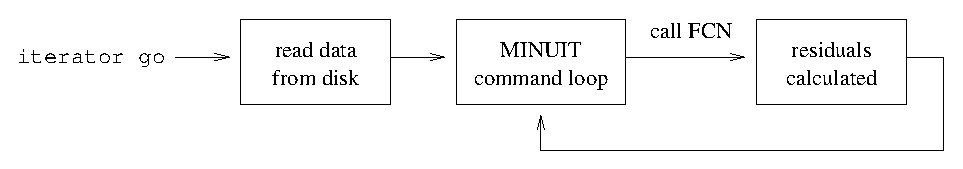
\includegraphics[width=\linewidth]{sketch.eps}
\end{center}

The ZDAlignmentMod module is built from three classes.
\begin{itemize}

  \item {\bf ZDAlignmentMod} declares parameters, loads tracks and
  hits, performs all hit-level cuts except the bad wire cut, and then
  invokes MINUIT interactive mode.

  \item The tracks that are loaded from the event stream have only
  been singly-fit, so {\bf ZDAlignmentDualTrackConstraint} is called
  to perform the dual-track constraint before storing the dual tracks
  into memory.  (Unlike the dual-track constraint in
  HelixIntersection, this one implements a full five-parameter fit.)

  \item Through the magic of MinuitInterface, MINUIT is given
  {\bf ZDAlignmentFcn} as its FCN.  This class actually stores the
  tracks and hits, opens the HistogramViewer window, declares
  histograms, calls ZD geometry objects to calculate residuals, fills
  those histograms, and writes out {\tt state.*} and {\tt best.*}.

\end{itemize}

Don't be confused by the fact that {\bf ZDAlignmentMod} and {\bf
ZDAlignmentFcn} both have {\tt iterate()} methods.  {\tt
ZDAlignmentMod::iterate()} is what gets called when you {\tt iterator
go}, and {\tt ZDAlignmentFcn::iterate()} is what gets called by
MINUIT.  They are completely different and have nothing to do with one
another.

\subsection{A walk through the ZDAlignmentMod code}

Before stepping through the code, I want to point out which essential
parts of the process are contained in other libraries, in case you're
looking for them.

\begin{itemize}

  \item The algorithm which minimizes the residual RMS when you type
  {\tt mini}, and the whole command loop itself, is in MINUIT, not
  ZDAlignmentMod.  Perhaps you knew this.

  \item When ordinary tracks are dual-fit, the application of that
  constraint happens in HelixIntersection.
  {\bf ZDAlignmentDualTrackConstraint} only defines equations that
  would be satisfied by a completely constrained pair of tracks and
  the derivatives of those equations with respect to track parameters.
  The application of the constraint happens in
  {\bf ZDAlignmentDualTrackConstraint}'s superclass when the inherited
  {\tt applyConstraint()} method is called.

  \item Whenever constants (like the ZD geometry parameters) are
  changed, the whole suez world (including AZDSenseWireStore) needs to
  be made aware of that update, or new calculations of residuals will
  yield old results.  Because the author of the iterator module
  superclass was expecting an event loop to follow any constants
  update, suez is only updated when you set a FIFrameIterator using
  the ``='' operator.  (As one might at the beginning of a {\tt for}
  loop over events.)

  But ZDAlignmentMod loops over the data stream only once.  After each
  change to the geometry constants, I create a new FIFrameIterator and
  set it equal to a FIFrameIterator pointer I have stored for this
  purpose, like this:
  \begin{center}
    \tt FIFrameIterator itFrame = *m\_frame;
  \end{center}
  It doesn't matter which event {\tt itFrame} points to, but this line
  is needed to update the ZD geometry in AZDSenseWireStore.

\end{itemize}

\subsubsection{A walk through {\tt ZDAlignmentMod::iterate()}}

When the user types {\tt iterator go} on the suez command line, the
function {\tt ZDAlign}- {mentMod::iterate(const FIFrameIterator\&
iBegin, iEnd)} is executed.  If this is the first time (i.e.\ the user
didn't exit the MINUIT command loop and type {\tt iterator go} a
second time), the module will load the two constants files: the
ZDGeomAlignment file pointed to by the ``geom'' parameter and the
AZDGeomLayer file pointed to by ``geomLayer.''  {\tt m\_geometry} and
{\tt m\_geomlayer} are CLEOConstantsModifiable objects, and they're
connected to the suez world by FIHolders, registered in
ZDAlignmentMod's constructor.  As soon as {\tt itFrame = *m\_frame} is
executed, any extraction of ZDGeomAlignment or AZDGeomLayer will get
the values in {\tt m\_geometry} and {\tt m\_geomlayer}.

Also on the first {\tt iterator go}, MINUIT is given parameter values
from the ZDGeomAlignment constants.  Only the first line (indexed by
{\tt [0]} in the code and 1 in the text file) is used because the
first line describes bulk alignment.  Lines {\tt [1]} and {\tt [2]} (2
and 3) describe internal alignments of the east and west endcaps.

Outside the {\tt m\_first\_time} conditional, {\tt m\_fcn.reset(iBegin)}
is called.  {\tt m\_fcn} is the only instance of {\bf ZDAlignmentFcn},
which is a MinuitInterface MIFcn, loaded into MINUIT in
ZDAlignmentMod's constructor.  It has two divers functions: it deletes
all memory-resident tracks and hits so it will be ready for a new set,
and it keeps track of the first Frame pointer, so that
{\bf ZDAlignmentFcn} can call {\tt itFrame = *m\_frame} all by itself.

Next is the loop over FIFrameIterators; this part looks more like a
typical processor.  FATables and FAItems are extracted from the
Frames, and there are subloops over tracks and hits.

The first thing that happens in this loop is a call to another
multifaceted function in {\bf ZDAlignmentFcn}--- this one is named
{\tt book()} because one of the things it might do is book histograms.
The only thing it will always do is notify {\bf ZDAlignmentFcn} of
possible new values of the ``showPlots'' and ``fakeDriftFunctions''
parameters.  Everything else is only done if this is the first call to
{\tt book()}:
\begin{enumerate}

  \item {\bf ZDAlignmentFcn} will read AZDGeomLayer to find the
  original wire radii.  It needs to keep track of them in case the
  user alters these constants using the parameters {\bf radius} and
  {\bf del\_rad\_45}.  (E shouldn't.)

  \item {\bf ZDAlignmentFcn} will book the seven histograms.

  \item {\bf ZDAlignmentFcn} will initialize Qt and the
  HistogramViewer window.  It is at this point in the code that
  control is given to the user, who needs to open and arrange
  histogram subwindows, and then press ``Continue.''

\end{enumerate}

Back in {\tt ZDAlignmentMod::iterate()}, tracks, ZD hits, and the
magnetic field are extracted from the Frame (ultimately from the PDS
file).  ZDAlignmentBhabhaFilterProc should have already filtered out
all events with more or less than two tracks in each event, so
ZDAlignmentMod assumes there are two.  If there are fewer,
{\tt ++two} will segmentation fault and if there are more,
{\tt ZDAlignmentDualTrackConstraint::con}- {straint()} will assert.
(There will also be an assertion if the track reference points are at
different places.  Inward or ChisqFit tracks should always have a
reference point of (0, 0, 0).)  The two tracks are copied as
HIFitHelixes, because this is what HIFitConstraint uses internally.

The dual-track constraint is declared and applied in two lines: the
first constructs a temporary {\bf ZDAlignmentDualTrackConstraint}
object (this is what MagneticField is needed for), and the second
executes the dual-track fit.  {\bf ZDAlignmentDualTrackConstraint}
defines the constraint as an STL\_VECTOR of five constraint equations:
\begin{itemize}

  \item $\mbox{$d_0$}^{\mbox{\scriptsize track 1}} +
         \mbox{$d_0$}^{\mbox{\scriptsize track 2}} = 0$

  \item $\mbox{$z_0$}^{\mbox{\scriptsize track 1}} -
         \mbox{$z_0$}^{\mbox{\scriptsize track 2}} = 0$

  \item $\bullet$ $\,\bullet$ $\langle p_x \mbox{, } p_y \mbox{, } p_z \rangle =
         \langle -15 \mbox{MeV, } 0 \mbox{, } 0 \rangle$

\end{itemize}
The right-hand side fo the last constraint is not $\langle$0, 0,
0$\rangle$ because the two incident beams are slightly crossed in the
X-Z plane, and 15 MeV is the virtual photon momentum.  This number
comes from a measurement on $\psi(3770)$ data--- if the crossing angle
or beam energy changes, this should be reevaluated.  (If this value is
wrong, you would see a wave in ZDAlignmentBhabhaFilterProc's ``tracks
momentum phi'' histogram.)

These constraints are expressed as a method of
{\bf ZDAlignmentDualTrackConstraint}, {\tt constraint()}, which maps
track parameters to a vector which is $\langle$0, 0, 0, 0, 0$\rangle$
when the constraints are satisfied.  Another method,
{\tt constraintDerivatives()}, maps track parameters to a matrix of
partial derivatives $\partial \mbox{constraint} / \partial
\mbox{track-parameter}$ for the dual track fitter.  Be aware that
while STL\_VECTORs index with square brackets, starting with zero,
HepMatrixes index with parentheses, starting with one.  I tried to
make the difference in indexing explicit with a {\tt const int
offset}.

{\bf ZDAlignmentDualTrackConstraint} is the only part of
ZDAlignmentMod that depends on the magnetic field, and the way it does
so is not even strictly necessary.  The magnetic field is used to
convert track curvatures into momenta.  If the constraint merely
required the two tracks to have equal and opposite momenta, this
factor of magnetic field would be irrelevant--- instead of
constraining momentum, I could have constrained momentum$/$magnetic
field magnitude.  The normalization is only important for comparison
with crossing angle, because I expressed it in MeV.  There are other
ways to express a crossing angle (most of them in radians), but ``the
momentum of the virtual photon'' is the most unambiguous and
easiest-to-measure way of describing it that I am aware of, so this is
how I coded it.  Just be aware that this introduces an implicit
dependence on beam energy.

Back in {\tt ZDAlignmentMod::iterate()}, the dual-track constraint has
just been applied, and now it is time to drop events if their
dual-$\chi^2$ is too high.  (High dual-$\chi^2$s are strongly
correlated with high $|p_z|$: initial state radiation in one of the
incident beams gives the bhabha event a $z$-boost.)  Both
dual-constrained tracks are passed through a tighter cut on
$\cot(\theta)$.  (Yes, the one on the second track is redundant.)

Next is a loop over the two tracks, and within that, a loop over all
ZD hits on those tracks.  Temporary vectors of hits and signed drift
distances are filled if the hits pass {\tt kFITTABLE}, drift distance,
and layer-number cuts.  If, after these cuts, a track has any ZD hits
left, the track, hits, signed drift distances, and the average (ZD)
charge on the track are passed to {\bf ZDAlignmentFcn}, so that it can
insert these data into its vectors.

{\bf ZDAlignmentFcn} fills its vectors with a terrifying {\tt fill()}
method.  Instead of creating structures, I just made sure that vectors
containing information for the same event had the same indices.  There
is one average charge per track, but possibly more than one hit and
signed drift distance, so the latter need to be declared as vectors of
vectors.  Moreover, to avoid impicit calling of vector and
{\tt CalibratedZDHit} constructors, the elements of these nested
vectors need to be pointers to vectors and hit objects, rather than
the objects themselves.  Consequently, {\tt fill()} is rife with
referencing and dereferencing.  A lot of this structure could have
been hidden with type declarations, but I think it is clearer to
include all the asterisks.

{\tt ZDAlignmentMod::iterate()} ends with a call to MINUIT--- usually
a call to enter the command loop ({\tt m\_minuit->interact()})--- but
if the parameter ``interactive'' is false, MINUIT goes right into
minimization ({\tt m\_minuit->runMigrad()}).  In either case, MINUIT
takes over, and ZDAlignmentMod is only ever given control again when
{\tt ZDAlignmentFcn::iterate()}, the suez implementation of FCN, is
called.  If the user types ``show par'', this happens right away.

\subsubsection{A walk through {\tt ZDAlignmentFcn::iterate()}}

When MINUIT calls FCN, the function
{\tt ZDAlignmentFcn::iterate(double* v)} is executed.  The array
{\tt v} holds the thirteen current trial parameter values.
{\bf ZDAlignmentFcn} immediately sets the CLEOConstantsModifiable
objects to these values and prints them out to
{\tt state.zdgeomalignment} and {\tt state.pars}.  Then
\begin{center}
FIFrameIterator itFrame = *m\_frame;
\end{center}
is executed, and suez is notified of the changes.  The ZD hit
corrector, AZDSenseWireStore, and ZD gas description are re-extracted
from the Frame (which points uselessly at the first event).  I only
expect AZDSenseWireStore to differ with each change to the geometry
constants.

Next, the histograms are reset.  If this segmentation faults, or if
histograms are not being reset properly, you probably need to get a
post-Oct15\_03\_MC change to HbookHistogram which corrects a bug in
{\tt reset()}.

Next comes a nested loop over tracks and hits.  In the track loop,
four vectors need to be iterated-over simultaneously: {\tt m\_track},
{\tt m\_charge}, {\tt m\_vect}, and {\tt m\_drifts}.  A {\tt while}
loop checks for the end of the {\tt m\_track} vector, and immediately
asserts if the other three haven't reached their ends.  All four
iterators are incremented at the end of the {\tt while} loop.  Two of
these, {\tt m\_vect} and {\tt m\_drifts}, are vectors of vectors:
iteration over the second level in this hierarchy is the hit loop.
This loop is implemented the same way: a {\tt while} with an assertion
at the beginning and incrementation at the end.  If you're adding
structure, like another variable to be stored alongside tracks or
hits, be very careful to include all the necessary parts--- a missing
incrementor would be a silent bug.  (New variables must be correctly
deleted in {\tt reset()}, inserted in {\tt fill()}, have iterators
initialized before the {\tt while} loop, assertions at the beginning
of the {\tt while} block, and incrementors at the end of the
{\tt while} block.)

Bad wires are cut at the beginning of the hit loop, though they might
as well be dropped in {\tt ZDAlignmentMod::iterate()} with the other
hit-level cuts.  (Then they wouldn't even be loaded into memory, which
would be a good thing.)

Next, {\bf ZDAlignmentFcn} projects its local copy of the track helix
to a single ZD hit.  The standard routines for doing this were written
for track fitters; our job is much simpler, but we can re-use many of
the same routines.
\begin{center}
  \begin{tabular}{l p{0.41\linewidth} c | c p{0.41\linewidth}}
    & A normal track fitter & & & {\bf ZDAlignmentFcn} \\\hline
      1.
    &
      Create a HIZDSurfaceFactory and apply it to the current event.
      (This requires the tracks to have come from the Frame.)
    & & &
      Create a vector of HIIntersectionSurfaces and fill it with one
      HISingleWireCylinder pointer.
    \\
      2.
    &
      Create a HIHelixIntersector, feed it the surfaces, and tell it
      to sort them in increasing radius.
    & & &
      Create a HIHelixIntersector, feed it the surfaces (one surface),
      and tell it to not bother sorting.
    \\
      3.
    &
      Use {\tt swimToCurrentSurface()} to loop over surfaces, and
      process the hit at each stop.  The helix's reference point is
      implicitly moved to the point of closest approach to each hit.
    & & &
      Explicitly move the track's reference point close to the hit so
      that swimming is a smaller extrapolation.  Call
      {\tt swimToCurrentSurface()} once.
  \end{tabular}
\end{center}
\begin{center}
  \begin{tabular}{l p{0.41\linewidth} c | c p{0.41\linewidth}}
      4.
    &
      At each hit, execute {\tt applyTrack}- {\tt Corrections()} to apply
      corrections to the hit which require knowledge of the track.
    & & &
      Execute {\tt applyTrackCorrec}- {\tt tions()} to apply corrections to
      the hit which require knowledge of the track.
    \\
  \end{tabular}
\end{center}

This is where signed drift distances and average track charges are
needed: they are given to HISingleWireCylinder's constructor.  (Kalman
and ChisqFitter keep track of this extra information with a
{\tt HIZDSurfaceFactory::ZDHitAndDriftDistance} list.)  These signed
drift distances carry one more bit of information than the
{\tt distance()} you can get from CalibratedZDHit: the sign they are
given comes from a collection of algorithms in DoitProd which use
neighboring hits to determine which side of the wire a given drift
measurement came from.  This sign assignment is far more accurate than
assuming the drift measurement is from the same side as the projected
distance of closest approach.  I don't know what is done with the
average track charges, and I don't know if averaging over the charges
of only ZD hits is sufficient.

Once the track has been swum and track-dependent hit corrections
applied, many variables are extracted from the intersector, surface,
hit, and swum helix, and these are used to fill the histograms.  It is
entirely likely that new histograms will be needed in the future; this
is where their contents will be calculated.  If the user turns on the
``fakeDriftFunctions'' parameter, this is where the carefully
calculated signed drift distance is tossed in favor of a linear
extrapolation.  This could easily be modified to inherit the sign from
the track finder.

Lastly, the HISingleWireCylinder created with a {\tt new} operator
must be deleted before the end of the hit loop, to prevent a massive
memory leak.

After the track and hit loops, the histograms have all been refilled,
so it is time to draw them on the screen.  (This execution of the Qt
application gives the user zero milliseconds to move any subwindows
around--- if it did wait for the user, minimizations would take longer
than they would have to.)

The root-mean-square residual is calculated, and, if it is better than
any {\bf ZDAlignmentFcn} has seen so far, {\bf ZDAlignmentFcn} will
print all the pertinent parameters to {\tt best.zdgeomalignment} and
{\tt best.pars}.  This RMS is then returned to MINUIT, and MINUIT may
decide to sample another set of parameters and try again.

\section{DRAlignmentMod {\normalsize (and DRAlignmentBhabhaFilterProc)}}

\subsection{Differences in DRAlignmentMod Strategy}

Until now, we have been discussing the problem of how to find the
correct alignment of a solid object--- the ZD--- from residuals of
hits to tracks fitted in the DR.  DR alignment presents a slightly
different problem: the wedding cake, the part of the DR that needs to
be aligned, is made of eight distinct cake rings with two endplates
each, and all sixteen parts can move independently.  Fortunately,
because a DR wedding cake endplate only determines hit positions in
the X-Y plane, {\bf z} is neither measureable nor relevant.
Additionally, {\bf phix} and {\bf phiy} would only make small changes
to 2-D hit positions, so only three parameters are left per endplate.
If tracks are fit only to the DR stereo section, residuals in one cake
ring are completely independent of the alignment of any other cake
ring, so the problem splits up into eight independent ones, with only
six parameters each.
\begin{center}
  \begin{tabular}{c c}
%%     \begin{minipage}{0.45\linewidth}
%%       \begin{center}
%%         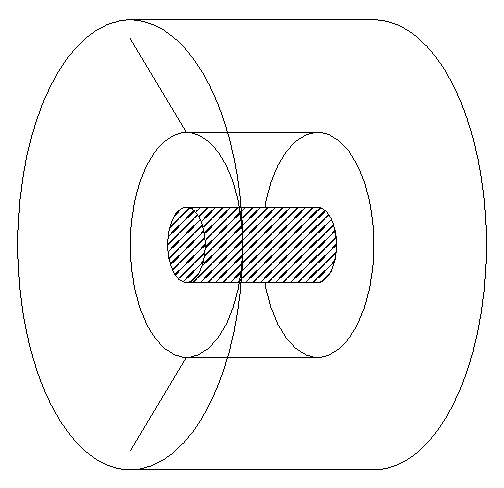
\includegraphics[width=0.3\linewidth]{loose_parts_ZD.eps}
%%       \end{center}
%%     \end{minipage} &
%%     \begin{minipage}{0.45\linewidth}
%%       \begin{center}
%%         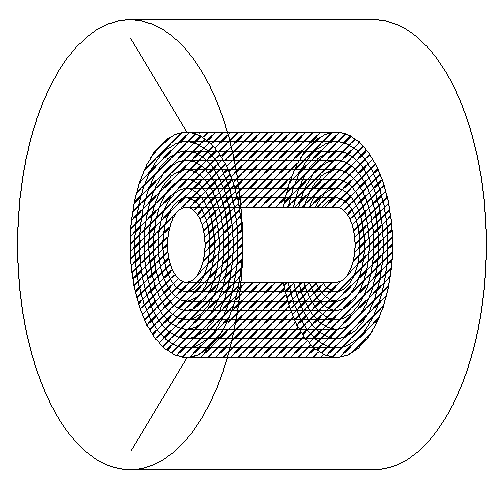
\includegraphics[width=0.3\linewidth]{loose_parts_DR.eps}
%%       \end{center}
%%     \end{minipage} \\
%%     & \\
    \hspace{0.45\linewidth} & \hspace{0.45\linewidth} \\
    {\bf ZD Alignment} & {\bf DR Alignment} \\\hline
    1 solid object & 16 solid objects \\
    1 alignment process & reducible to 8 independent alignments \\
    6 parameters & 3 parameters $\times$ 2 objects per alignment \\
  \end{tabular}
\end{center}
DR alignment has a different set of six parameters, and acts on only
one cake ring.
\begin{enumerate}

  \item {\bf xEast} is the offset of an east cake ring, in the
  direction along the floor and perpendicular to the beam axis.

  \item {\bf yEast} is the vertical offset of an east cake ring

  \item {\bf phiEast} is the distance the outer radius of an east cake
  ring is rotated around the beamline

  \item {\bf xWest} is the x offset of a west cake ring (west is the
  direction of incident positrons)

  \item {\bf yWest} is the y offset of a west cake ring

  \item {\bf phiWest} is the distance of a west cake ring rotation

\end{enumerate}

Beyond that, the procedure is remarkably similar.  Therefore, I made a
tool for DR alignment by copying ZDAlignmentMod and changing all
instances of ``ZD'' to ``DR.''  This may sound like a horrible cheat,
but it makes it easier for a new person to take over the project,
since the code is nearly the same.  Differences will evolve over time,
so someday knowledge of ZDAlignmentMod won't help someone understand
DRAlignmentMod, but I should hope alignment is a solved problem by
then!

A good introduction to DRAlignmentMod strategy is therefore Section
\ref{ZDAlignmentMod_Strategy}, ZDAlignmentMod Strategy (page
\pageref{ZDAlignmentMod_Strategy}).  The discussion of residuals,
drifts and dcas still apply because the DR is as much a wire chamber
as the ZD.  DRAlignmentMod loads tracks and hits from a pre-filtered
source (DRAlignmentBhabhaFilterProc) the same way and calls MINUIT for
its command loop.  DRAlignmentMod uses the same dual-track constraint,
though it defines its own constraint class,
{\bf DRAlignmentDualTrackConstraint} (which is exactly the same).  It
is still wise to use ChisqFitProd as a fitter, and the event
selections defined in DRAlignmentBhabhaFilterProc and DRAlignmentMod
are the same as in the ZDAlignment counterparts (except the
requirement for tracks with at least one ZD hit--- in the DR version,
at least eight axial DR hits are required).  By default, only
time-of-flight and signal-propogation corrections are applied to DR
hits.  This is the right thing for ZD hits, but perhaps the DR is
understood well enough that more track-dependent corrections may be
applied.

Most ZD hit selections have no analogue for the DR, so the only DR hit
selection that is applied is the drift distance cut: only DR hits
between 1.5 and 3.8 mm are passed.

The last issue is one of numerology: the axial section is composed of
eight wedding cake rings (the physical structure) and sixteen layers
(the sense wires).  Each cake ring has two sense wires--- two layers.
Cake rings and layers are both numbered in increasing radius: cake
ring 1 is closest to the beampipe and suspends sense wires in layers 1
and 2.  DRAlignmentMod has two {\tt const} functions for converting
from layers to cake rings: {\tt DRAlignmentMod::cake\_ring()} and {\tt
DRAlignmentFcn::cake\_ring()}.

\subsection{Differences in DRAlignmentMod Use}

\subsubsection{Differences in running DRAlignmentBhabhaFilterProc}

Just like ZDAlignmentMod, DRAlignmentMod expects tracks and hits to
come pre-reconstructed and pre-selected from a PDS file.  The event
filter for DR alignment is DRAlignmentBhabhaFilterProc, and, as stated
above, almost all the same cuts are applied.

Because we are now aligning the DR axial section, it is now necessary
to fit the tracks to the stereo section only, rather than the whole
DR.  (We should still leave the ZD out of the fit!)  It is a bit more
difficult to deweight part of a detector--- the DR axial section---
rather than a whole detector.  An example of how to do this is
illustrated by DRAlignmentBhabhaFilterProc/Test/sample.tcl and
DRAlignmentBhabhaFilterProc/Test/deweight\_axial.drweight2layerdriftentang.
If the fittingweights change, you will need to create a new deweighted
deweighted\_axial file from the new fittingweights. Here's how to do
it:
\begin{enumerate}

  \item Make a local copy of the latest DR fittingweights (bdl type
  DRWeight2LayerDrift- EntAng).  If these weights are in the database,
  you can use the constants website (page \pageref{constantsweb}).
  (Wherever you get them from, be sure to set the first two numbers to
  ``1 0'' so the file will be used for any run range.)

  \item Edit your local copy so that any line with a layer number
  (first column) from 1 to 16 has a very large fittingweight (last
  column).  1000 will do.  (Why a large number, rather than a small
  one?  See page \pageref{fittingweights} for an explaination.)  An
  awk commandline that will do this is:
  \begin{verbatim}
awk '(  $1>0 && $1<17 && $9!="DEFAULT" ){print $1 $2 $3 1000}
     (!($1>0 && $1<17 && $9!="DEFAULT")){print $0}
     < in.drweight2layerdriftentang > out.drweight2layerdriftentang \end{verbatim}

  \item Load this as the new fittingweights:
\begin{verbatim}
source_format sel DRWeight2LayerDriftEntAngFileSourceFormat
file in out.drweight2layerdriftentang \end{verbatim}

\end{enumerate}

In direct analogy to ZDAlignmentMod, DRAlignmentMod needs the
following data to run:
\begin{itemize} \renewcommand{\labelitemi}{$-$}
  \item FAItem$<$DBEventHeader$>$
  \item FAItem$<$DBTrackerValues$>$
  \item FATable$<$TRTrack$>$
  \item FATable$<$TRHelixPionFit$>$
  \item FAItem$<$SeedTrackDRHitLattice$>$
  \item FATable$<$CalibratedDRHit$>$
\end{itemize}

\subsubsection{Differences in running DRAlignmentMod}

Like ZDAlignmentMod, DRAlignmentMod will require a starting
geometry--- bdl type DRGeomAlignment--- which you can get from the
same website (page \pageref{constantsweb}).  Be sure to set the first
two numbers to ``1 0'' so the file will be used for any run range.
Point DRAlignmentMod to that file with ``geom'' in the same way.
DRAlignmentMod doesn't provide any naughty parameters that shift wire
position radius or wire sag, so no ADRGeomLayer is needed.

Even though they look superficially similar, the DRGeomAlignment
constants are interpreted very differently from their ZD counterparts.
\begin{center}
  \begin{tabular}{p{0.45\linewidth} p{0.45\linewidth}}
    ZDGeomAlignment indices & DRGeomAlignment indices \\\hline
    \begin{minipage}{\linewidth}
      \begin{tabular}{c l}
        1 & Bulk alignment \\
        & \\
        2 & East endcap alignment \\
        & \\
        3 & West endcap alignment \\
      \end{tabular}
    \end{minipage} &
    \begin{minipage}{\linewidth}
      \begin{tabular}{c l}
        1 & DR bulk alignment \\
        2 & East stereo endplate \\
        \begin{tabular}{c} 3 \hspace{0.1 cm} \\ \vdots \hspace{0.1 cm} \\ 10 \hspace{0.1 cm} \end{tabular} &
          $\Bigg\}$ East cake rings 1--8 \\
        \begin{tabular}{c} \hspace{0 cm} 11 \\ \hspace{0 cm} \vdots \\ \hspace{0 cm} 18 \end{tabular} &
          $\Bigg\}$ West cake rings 1--8 \\
      \end{tabular}
    \end{minipage} \\
  \end{tabular}
\end{center}
Also, while ZDGeomAlignment is in normal CLEO-III units (meters and
radians), DRGeomAlignment is completely in inches.  The three angles,
{\bf phix}, {\bf phiy}, and {\bf phiz} are in inches at the outer
radius of the cake ring.  Internally, DRAlignmentMod uses only
millimeters, and it does all the conversions from constants/files to
MINUIT and back to constants/files correctly.  There are two problems
with this situation: everything the user sees in MINUIT is an awkward
factor of 25.4 different from what e sees in the constants files, and
the angles are still in a wierd unit: millimeters at the outer radius.

When you run the corresponding {\tt align.tcl}, be aware that it sets
a new parameter called ``ring.''  This specifies which cake ring
number you will be aligning.  One way to align all eight is to start
with ``ring'' set to 1, enter the MINUIT command loop with
{\tt iterator go}, do an alignment, exit MINUIT with {\tt exit} (don't
{\tt exit} twice!), set the ``ring'' parameter to 2, enter MINUIT again,
etc.  {\tt state.*} and {\tt best.*} will include cumulative changes.
If you encounter a crash partway through, load
{\tt state.drgeomalignment} or {\tt best.drgeomalignment} with
``geom'' to return to your last or best alignment.

But perhaps you don't have this kind of patience--- suppose you want
to log into eight machines at the same time, align a different cake
ring in each, and then collect results.  This can be done in principle
because calculations of residuals of one cake ring are independent of
the alignment of other cake rings.  But all of your jobs would be
printing their latest and best states to the same files--- you would
need to edit {\tt DRAlignmentFcn::iterate()} (near lines 266 and 398
of DRAlignmentFcn.cc) to print out different file names depending on
the value of {\tt int m\_ring}.  You would then have to merge the
outputs of the eight files.

Like ZDAlignmentMod, DRAlignmentMod has two extra parameters for
faking drift functions with a straight line:
\begin{enumerate}\setcounter{enumi}{6}
  \item {\bf t0} --- offset time
  \item {\bf drift} --- drift velocity
\end{enumerate}
but it doesn't have all the others.  This is because I don't expect
the others to be useful, so I didn't want to port them to a
DR-alignment context.

DRAlignmentMod has one fewer histogram than ZDAlignmentMod: ``V
layer'' (residual versus layer) is not useful for DR alignment because
it measures a difference between U layers and V layers; the axial
section of the DR has neither.  All the other histograms are the same.
Even the three ``V phi'' histograms have the same $\cot(\theta)$ cuts
as their ZD counterparts, but they are labelled ``east,'' ``mid,'' and
``west'' to help you determine whether you should shift the east
endplate or the west endplate to cancel a distortion.

These are all the differences between DR and ZD alignment tools as of
\today.  Others are bound to appear as DRAlignmentMod becomes better
specialized to its unique task.  Be sure to check the CVS log for
names other than mine!

\section{DualTrackProd {\normalsize (and DualTrackToUsageTagProd)}}
\label{dualtrackprod}

One part of ZD- and DRAlignmentMod is a new dual-track constraint
(described in Section \ref{dualconstraint} on page
\pageref{dualconstraint}).  This constraint differs from the one used
in silicon alignment in that it is a five parameter constraint (the
old one didn't constrain $p_z$), crossing angle is now expressed as a
momentum shift, and perhaps most importantly, hit residuals are
calculated with the new dual-tracks.  When it became clear that this
new constraint would be useful in other alignment and calibration
work, I wrapped it in a producer so that it is easily accessible in
suez.

A number of technical issues made it easier to replace the existing
structure than to modify it, although this raises the possibility of
name confusion.  These are the old and new names (middle and right,
respectively):
\begin{center}
  \begin{tabular}{p{0.3\linewidth} | p{0.3\linewidth} | p{0.3\linewidth}}
    \begin{minipage}{\linewidth} HIFitConstraint subclass \end{minipage} &
      \begin{minipage}{\linewidth} HelixIntersection/HIDual- TrackConstraint \end{minipage} &
        \begin{minipage}{\linewidth} DualTrackProd/DualTrack- Constraint \end{minipage} \\
    & & \\
    \begin{minipage}{\linewidth} Extractable object \end{minipage} &
      \begin{minipage}{\linewidth} DualTrackHelices/Dual- TrackHelices (FATable) \end{minipage} &
        \begin{minipage}{\linewidth} DualTrackProd/DualTrack (FAItem) \end{minipage} \\
    & & \\
    \begin{minipage}{\linewidth} Producer \end{minipage} &
      \begin{minipage}{\linewidth} DualTrackHelicesProd \end{minipage} &
        \begin{minipage}{\linewidth} DualTrackProd \end{minipage} \\
    & & \\
    \begin{minipage}{\linewidth} Conversion to standard helix and lattice objects \end{minipage} &
      &
        \begin{minipage}{\linewidth} DualTrackToUsageTagProd \end{minipage} \\
  \end{tabular}
\end{center}

The constraint in DualTrackProd is a cut-and-paste copy of the one in
ZDAlignmentMod.  While ZDAlignmentMod and DRAlignmentMod are both
sinlge-use tools, and therefore meant to be very open to modification
and replaced when they become too hairy to work with, DualTrackProd is
a finished product--- we should think of the code in DualTrackProd as
the original and the alignment modules as containing temporary copies.
The best thing would be to rewrite the AlignmentMods to extract
dual-track objects from DualTrackProd, rather than defining their own,
but I haven't done this because they are just temporary, after all.

\subsection{How to Use DualTrackProd}

Before describing the various methods of extracting dual-tracks, I
want to warn you that the specification of the crossing angle depends
on beam energy.  The default crossing angle DualTrackProd uses is 15
MeV in the $-\hat{x}$ direction, which comes from a measurement at
$\psi(3770)$.  If your bhabhas are above 4270 or below 3270 MeV, it
would be wise to re-measure the crossing angle with the ``printOutP''
parameter described on page \pageref{printOutP}.

\subsubsection{Extracting via special DualTrack types}

If you are building a new processor/producer, here's the simplest way
to get dual-tracks:
\begin{enumerate}

  \item Load DualTrackProd in your tcl script with {\tt prod sel
  DualTrackProd}.

  \item Include {\tt "DualTrackProd/DualTrack.h"} in your {\tt .h} or
  {\tt .cc}.

  \item Extract a DualTrack object from the event stream:
\begin{verbatim}FAItem<DualTrack> dual_track;
extract(iFrame.record(Stream::kEvent), dual_track); \end{verbatim}

\end{enumerate} \begin{itemize}

  \item If this event successfully performed a dual-track fit,
  {\tt dual\_track->results().fit}- {\tt Successful()} will be true.  (You
  don't need to pre-select two-track events--- unsuitable events will
  just have a false {\tt fitSuccessful()} flag.)

  \item If {\tt dual\_track->results().fitSuccessful()} is true, two
  methods will return DualTrackFitHelix objects:
  {\tt dual\_track->positive()} and {\tt ->negative()}.
  These two objects are tracks (DualTrackFitHelix son of HIFitHelix
  son of HIHelix is a son of KTHelix), so you can ask for things like
  {\tt positive().cotTheta()}.

  \item The quality of the dual-fit can also be found by
  {\tt results().chisq()} divided by {\tt results().ndof()}.

\end{itemize}

If you'd rather loop over tracks, you can extract a table of
DualTrackFitHelixes.
\begin{enumerate}\setcounter{enumi}{2}

  \item \begin{verbatim}FATable<DualTrackFitHelix> dual_tracks;
extract(iFrame.record(Stream::kEvent), dual_tracks);
for (FATable<DualTrackFitHelix>::const_iterator dualItr =
         dual_tracks.begin();
     dualItr != dual_tracks.end();
     ++dualItr) {\end{verbatim} \hspace{2 cm} $\ddots$

\end{enumerate}
These two helices are the same as {\tt dual\_track->positive()} and
{\tt ->negative()}.  Incidentally, these have the same
{\tt identifier()}s as the singly-fit tracks they correspond to, so
you can do things like {\tt navtracks.find(dualItr.identifier())}.

DualTrackProd will also calculate residuals of hits with respect to
the dual-constrained tracks.
\begin{enumerate}\setcounter{enumi}{3}

  \item Extract the appropriate lattice (DR or ZD):
\begin{verbatim}FAItem<DualTrackZDHitLattice> dual_zdlattice;
extract(iFrame.record(Stream::kEvent), dual_zdlattice); \end{verbatim}

  \item Following the existing convention, tracks are on the left of
  the lattice, and hits are on the right.
\begin{verbatim}    // (in DualTrackFitHelix loop)
    const DualTrackZDHitLattice::Links& dual_zdlinks =
      dual_zdlattice->linksGivenLeft(dualItr->identifier());
    DualTrackZDHitLattice::Links::const_iterator dual_zdlinkItr =
      dual_zdlinks.begin();
    DualTrackZDHitLattice::Links::const_iterator dual_zdlinkEnd =
      dual_zdlinks.end();
    for (; dual_zdlinkItr != dual_zdlinkEnd;  ++dual_zdlinkItr) {
        const CalibratedZDHit::Identifier* hitId =
          (**dual_zdlinkItr).rightID();
        DualTrackZDHitLink& linkData = (**dual_zdlinkItr).linkData();
        linkData.residual();\end{verbatim}

\end{enumerate}

\subsubsection{Extracting via a usage tag}

If you have an existing processor/producer which already loads
singly-fit tracks and residuals and want to modify it to load
dual-constrained tracks and residuals instead, the above procedure
would be inconvenient because you would need to change all the type
names.  Here's an alternative way to get dual-tracks and -hits, which
will be easier to merge:
\begin{enumerate}

  \item Load these two producers in your tcl script:
\begin{verbatim}prod sel DualTrackProd
prod sel DualTrackToUsageTagProd \end{verbatim}

  \item No DualTrack include files are needed.

  \item Change TRHelixFit and FitDRHitLattice extractions to request
  the ``DualTrack'' usage tag.  The extract lines of
\begin{verbatim}FATable<TRHelixElectronFit> tracks;
FAItem<ElectronFitDRHitLattice> drlattice;
FAItem<ElectronFitZDHitLattice> zdlattice;
extract(iFrame.record(Stream::kEvent), tracks);
extract(iFrame.record(Stream::kEvent), drlattice);
extract(iFrame.record(Stream::kEvent), zdlattice); \end{verbatim}
  become
\begin{verbatim}extract(iFrame.record(Stream::kEvent), tracks, "DualTrack");
extract(iFrame.record(Stream::kEvent), drlattice, "DualTrack");
extract(iFrame.record(Stream::kEvent), zdlattice, "DualTrack"); \end{verbatim}

  It doesn't matter which mass hypothesis you extract--- the
  dual-track constraint is applied to one hypothesis and
  DualTrackToUsageTagProd fills all hypotheses with the same modified track.

\end{enumerate}

You can still extract a DualTrack object directly to get information
about the dual-$\chi^2$.

\subsubsection{Extracting via NavTrack with a production tag}

The situation becomes a bit more complicated if you're getting your
tracks and hits from NavTrack, because DualTrackProd gets its
singly-fit tracks from NavTrack.  But there's a way to do this, too:
you just need to load two instances of NavigationProd.

\pagebreak
Here's how to do that:
\begin{enumerate}

  \item Load all of the following into your tcl script.
\begin{verbatim}# This NavigationProd holds singly-fit tracks
prod sel NavigationProd
prod sel TrackDelivery

prod sel DualTrackProd
prod sel DualTrackToUsageTagProd

# Load a second NavigationProd to hold dual-fit tracks
prod sel NavigationProd production "DualTrack"
prod sel TrackDeliveryProd production "DualTrack"
param NavigationProd@DualTrack fitterUsageTag "DualTrack"
param TrackDeliveryProd@DualTrack fitterUsageTag "DualTrack" \end{verbatim}

  \item No DualTrack include files are needed.

  \item Now, instead of requesting a special usage tag, we extract a
  special production tag.
\begin{verbatim}FATable<NavTrack> navtracks;
extract(iFrame.record(Stream::kEvent), navtracks); \end{verbatim}
  becomes
\begin{verbatim}FATable<NavTrack> dual_navtracks;
extract(iFrame.record(Stream::kEvent),
                                 dual_navtracks, "", "DualTrack"); \end{verbatim}
  (In fact, you can extract both.)

\end{enumerate} \begin{itemize}

  \item Now you should be able to use the NavTrack conveniences.
\begin{verbatim}FATable<NavTrack>::const_iterator dual_navtrackItr =
    dual_navtracks.begin();
const FATable<NavTrack>::ZDHitLinkTable* dual_zdlinks =
    dual_navtrackItr->pionZDLinks(); \end{verbatim}

\end{itemize}

\subsection{Everything you want to know about DualTrackProd}

\subsubsection{DualTrackProd parameters}

Descriptions of the DualTrackProd parameters are also available
through the normal suez parameter help system.

\begin{itemize}

  \item ``massHypo'' allows you to pick which mass hypothesis to
  dual-constrain.  It is a string, and its value must be one of
  ``electron,'' ``muon,'' ``pion,'' ``kaon,'' ``proton,''
  ``exitElectron,'' ``exitMuon,'' ``exitPion,'' ``exitKaon,'' and
  ``exitProton.''

\pagebreak

  \item ``vphoPx''
  \item ``vphoPy''
  \item ``vphoPz'' allows you to set the 3-momentum of the virtual
  photon before it decays into back-to-back particles.  ``Px'' and
  ``Py'' physically correspond to a crossing angle of the incident
  beams, which is by default $\langle$ 15 MeV, 0 $\rangle$.  A
  non-zero ``Pz'' would arise from asymmetric beams, which are not
  available at CESR.

  Be careful of the sign convention here: it's wrong.  Considering
  that I'm calling this ``the virtual photon momentum'' rather than
  ``the virtual photon coordinate frame boost,'' it goes the wrong
  way.  I would fix it now, but people are already using it, so just
  print out the default value of ``vphoPx'' before changing it: that
  will tell you which way it goes.

  \item ``constrainPoint''
  \item ``constrainPT''
  \item ``constrainPZ'' are three options, true by default, which let
  you set the kind of constraint you want.  ``constrainPoint'' will
  force the impact parameters $d_0$ and $z_0$ of the two tracks to be
  the same, ``constrainPT'' will force the total transverse momentum
  to be consistent with 2D back-to-backness and the crossing angle,
  and ``constrainPZ'' will force the total longitudinal momentum to be
  zero.

  \item ``printOutP'' \label{printOutP} is a diagnostic option.  If
  you set this to true, DualTrackProd will print out the virtual
  photon 3-momentum for every two-track event, by adding the momenta
  of singly-fit tracks.  You can then put these into an ntuple or
  histogram to look for the peak in X-Y-Z (or eyeball it if you're
  brave).  If you are re-measuring the crossing angle because the beam
  energy has changed, ignore Y and Z.

\end{itemize}

\subsubsection{DualTrack member data}

These are all the public member functions of the DualTrack object.

\begin{itemize}

  \item {\tt const DualTrackFitHelix\& positive()}
  \item {\tt const DualTrackFitHelix\& negative()} return track
  helices for the positive and negative tracks used in the
  dual-constraint.  DualTrackFitHelix is a HIFitHelix, which is a
  HIHelix, which is a KTHelix.

  \item {\tt const DualTrackConstraint\& constraint()} returns the
  constraint object itself, which can be useful if you want to
  calculate the constraint values and derivatives yourself.  Be
  careful: the meanings of the output vector and matrix indices depend
  on the parameters ``constrainPoint,'' ``constrainPT,'' and
  ``constrainPZ.''

  \item {\tt const HIFitConstraint::Results\& results()} returns a
  results object.  A results object has these useful members (and
  more!):
  \begin{itemize}

    \item {\tt fitSuccessful()}

    \item {\tt deltaTrackParameters()}

    \item {\tt chisq()} is the dual-$\chi^2$.

    \item {\tt ndof()} depends on the parameters ``constrainPoint,''
    ``constrainPT,'' and ``constrainPZ,'' but doesn't vary from event
    to event.

  \end{itemize}

  \item {\tt const HepVector3D\& pVirtualPhoton()}
  \item {\tt DABoolean pointConstraint()}
  \item {\tt DABoolean ptConstraint()}
  \item {\tt DABoolean pzConstraint()} tell you the parameter values
  under which DualTrackProd is being run.

\end{itemize}

\subsubsection{DualTrackZDHitLink and DualTrackDRHitLink member data}

\begin{itemize}

  \item {\tt used()} is the same as the single-fit version (set by the
  fitter).

  \item {\tt residual()} is the measured drift $-$ dual-track
  predicted dca.

  \item {\tt residualError()} is the error in the measured drift
  only--- no contribution from {\tt signedDcaError()}.  This is what
  ChisqFitProd outputs, so I'm doing the same thing.

  \item {\tt momentum()} comes entirely from the curvature of the
  dual-track.  Because DualTrackProd doesn't know about $dE/dx$, this
  momentum is the same all along the track.

  \item {\tt trackRefPt()} is the point of closest approach of the
  dual-track to a given hit.

  \item {\tt signedDcaToWire()} is the distance of closest approach,
  predicted by the dual-track.

  \item {\tt signedDcaError()} is the uncertainty in the above.

  \item {\tt sinTrackToRadial()} is an approximation of the entrance
  angle using the dual-track.

  \item {\tt driftTime()} is the measured time--- exactly the same as
  the single-fit version.

  \item {\tt fittingWeight()} is the fittingweight assumed in the
  fit--- exactly the same as the single-fit version.

  \item {\tt signedDriftDistance()} is the measured drift distance---
  exactly the same as the single-fit version.

  \item {\tt singleTrack\_residual()}
  \item {\tt singleTrack\_residualError()}
  \item {\tt singleTrack\_momentum()}
  \item {\tt singleTrack\_trackRefPt()}
  \item {\tt singleTrack\_signedDcaToWire()}
  \item {\tt singleTrack\_signedDcaError()}
  \item {\tt singleTrack\_sinTrackToRadial()} all provide the user
  with access to what the singly-fit track determined for this hit.
  It's just a convenience.

\end{itemize}

\vfill
\begin{center}
Happy calibrating!
\end{center}
\vfill

\end{document}
